\documentclass[tikz,border=10pt]{standalone}
\usetikzlibrary{angles}
\begin{document}
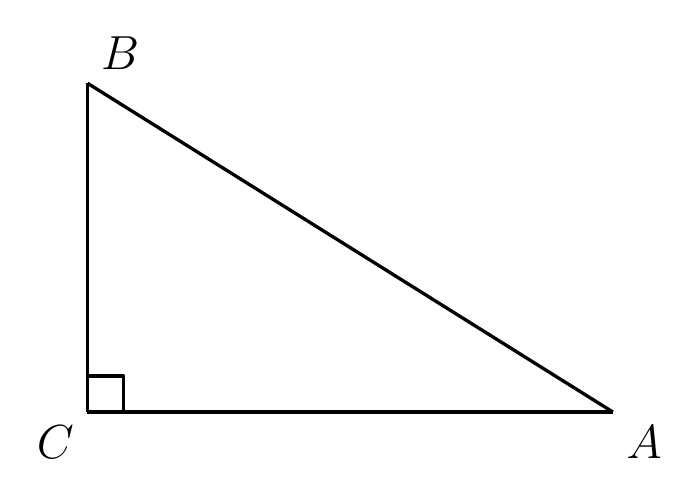
\begin{tikzpicture}[line width=1.2pt, line join=round]
\coordinate (A) at (3.311,-2.075);
\coordinate (B) at (-3.362,2.101);
\coordinate (C) at (-3.362,-2.075);




\draw (A) -- (B);
\draw (A) -- (C);
\draw (B) -- (C);


\draw pic[draw, angle radius=0.458cm] {right angle=A--C--B};


\node[above right=1pt] at (B) {\fontsize{17.5}{21}\selectfont $B$};
\node[below left=1pt] at (C) {\fontsize{17.5}{21}\selectfont $C$};
\node[below right=1pt] at (A) {\fontsize{17.5}{21}\selectfont $A$};
\end{tikzpicture}
\end{document}